\chapter{一元函数的导数及其应用}

本章介绍导数。导数是分析函数的一个系统化的工具,但不可偏重导数。

本章要点:
\begin{itemize}
    \item 导数。
\end{itemize}

\begin{tcolorbox}
导数是最后的工具,别啥都一上来求导!
\end{tcolorbox}

\newpage
\section{导数的概念及其意义}

本节要点:
\begin{itemize}
    \item 掌握导数的概念;
    \item 理解导数的几何意义。
\end{itemize}

%============================================================
\subsection{变化率的问题}

\begin{definition}[增量和变化率]
我们定义,{\bf 自变量的增量}是两个自变量的差,{\bf 因变量的增量}是两个因变量的差,即:
\begin{align*}
&\Delta x:=x_1-x_0 \\
&\Delta y:=y_1-y_0=f\left( x_1 \right) -f\left( x_0 \right)
\end{align*}
我们继续定义两个增量的比值为{\bf 函数的变化率},即:
\[
\frac{\Delta y}{\Delta x}=\frac{f\left( x_1 \right) -f\left( x_0 \right)}{x_1-x_0}=\frac{f\left( x_0+\Delta x \right) -f\left( x_0 \right)}{\Delta x}
\]
\end{definition}

显然,函数的变化率是一个和自变量及其增量区间有关的新函数。当取相同的$\Delta x$时,变化率描述了函数的变化快慢。变化率越大,说明函数在同等$\Delta x$下的变化越大。

%============================================================
\subsection{导数的概念及其几何意义}

下面我们考察函数在一个点上的变化率,即当$x_1\rightarrow x_0$(或$\Delta x\rightarrow 0$),函数的变化率的存在性和取值。

\begin{definition}[导数]
设函数$f\left( x \right) $在点$x_0$的某邻域$N\left( x_0 \right) $内有定义,若当$\Delta x\rightarrow 0$时$\Delta y/\Delta x$的极限存在,则称{\bf 函数$f\left( x \right) $在$x_0$处可导},并称此极限值为{\bf 函数$f\left( x \right) $在点$x_0$的导数(derivative)},记为$f'\left( x_0 \right) $,即:
\[
f'\left( x_0 \right) :=\underset{\Delta x\rightarrow 0}{\lim}\frac{\Delta y}{\Delta x} \quad \text{或} \quad f'\left( x_0 \right) :=\underset{x_1\rightarrow x_0}{\lim}\frac{f\left( x_1 \right) -f\left( x_0 \right)}{x_1-x_0}
\]
也可用莱布尼兹(Leibniz)记号记为:
\[
\left. y' \right|_{x=x_0} \quad \text{或} \quad \left. \frac{dy}{dx} \right|_{x=x_0}
\]
\end{definition}

从定义上来讲,函数$f\left( x \right) $在$x_0$处的导数是一个极限,是一个可计算的确定的数。具体还有左导数和右导数,略。

\begin{definition}[导函数]
如果函数$f\left( x \right) $在区间$D$内每一点都可导,则称每个导数构成的新函数为{\bf $f\left( x \right) $的导函数},记为$f'\left( x \right) $(或$y'$)。显然,导函数$f'\left( x \right) $在$x_0$的值就是导数$f'\left( x_0 \right) $。
\end{definition}

除非特别指明,一般我们将导函数简称为导数。区间$\left( a,b \right) $(或$\left[ a,b \right] $)内所有可导函数的集合通常记作$D\left( a,b \right) $(或$D\left[ a,b \right] $),所以$f\left( x \right) $在区间$D$内可导也可记作$f\left( x \right) \in D\left( a,b \right) $(或$f\left( x \right) \in D\left[ a,b \right] $)。

求导是对函数的一种运算。运算对象是函数,得到的结果是另一个函数。从集合角度,求导是一个函数集合到另一个函数集合的映射。

\begin{tcolorbox}
在讨论导数的时候,紧紧抓住导数的定义,从定义出发。后续关于导数的定理和公式都是用定义证明和推导。
\end{tcolorbox}

从几何上来讲,导数的意义是切线的斜率。物理上,导数描述了一个物理量的瞬时变化速度,比方说路程的导数是速度,速度的导数是加速度。导数为求解物理量的变化速度提供了强大的数学工具。






\newpage
\section{导数的运算}

本节要点:
\begin{itemize}
    \item 掌握基本初等函数的求导公式;
    \item 掌握导数的运算法则;
    \item 掌握复合函数的求导方法。
\end{itemize}

%============================================================
\subsection{基本初等函数的导数}

\begin{align*}
\begin{matrix}
	\left( C \right) '=0 \hfill                                       & \left( x^a \right) '=a\cdot x^{a-1} \hfill \\
	\left( a^x \right) '=a^x\ln a \hfill                              & \left( e^x \right) '=e^x \hfill \\
	\left( \log _ax \right) '=\frac{1}{x\ln a} \hfill                 & \left( \ln x \right) '=\frac{1}{x} \hfill \\
	\left( \sin x \right) '=\cos x \hfill                             & \left( \cos x \right) '=-\sin x \hfill \\
	\left( \tan x \right) '=\sec ^2x \hfill                           & \left( \cot x \right) '=-\csc ^2x \hfill \\
	\left( \sec x \right) '=\sec x\cdot \tan x \hfill                 & \left( \csc x \right) '=-\csc x\cdot \cot x \hfill \\
	\left( \mathrm{arc}\sin x \right) '=\frac{1}{\sqrt{1-x^2}} \hfill & \left( \mathrm{arc}\cos x \right) '=-\frac{1}{\sqrt{1-x^2}} \hfill \\
	\left( \mathrm{arc}\tan x \right) '=\frac{1}{1+x^2} \hfill        & \left( \mathrm{arc}\cot x \right) '=-\frac{1}{1+x^2} \hfill \\
	\left( \mathrm{sh}x \right) '=\mathrm{ch}x \hfill                 & \left( \mathrm{ch}x \right) '=\mathrm{sh}x \hfill \\
\end{matrix}
\end{align*}

以上基本公式中,除了$\left( C \right) ',\left( a^x \right) ',\left( \sin x \right) '$,其余都可以从这三个公式导出。

{\bf 计算$\left( C \right) '$}
\[
\left( C \right) '=\underset{\Delta x\rightarrow 0}{\lim}\frac{C-C}{\Delta x}=0
\]

{\bf 计算$\left( a^x \right) '$}
\[
\left( a^x \right) '=\underset{\Delta x\rightarrow 0}{\lim}\frac{a^{x+\Delta x}-a^x}{\Delta x}=a^x\underset{\Delta x\rightarrow 0}{\lim}\frac{a^{\Delta x}-1}{\Delta x}=a^x\ln a
\]

{\bf 计算$\left( \sin x \right) '$}
\begin{align*}
\left( \sin x \right) '&=\underset{\Delta x\rightarrow 0}{\lim}\frac{\sin \left( x+\Delta x \right) -\sin x}{\Delta x} \\
&=\underset{\Delta x\rightarrow 0}{\lim}\frac{2\sin \frac{\Delta x}{2}\cos \frac{2x+\Delta x}{2}}{\Delta x}=\underset{\Delta x\rightarrow 0}{\lim}cos \frac{2x+\Delta x}{2}=\cos x
\end{align*}

%============================================================
\subsection{导数的四则运算法则}

\begin{align*}
&\left( C\cdot f \right) '=C\cdot f' \\
&\left( f\pm g \right) '=f'\pm g' \\
&\left( f\cdot g \right) '=f'g+fg' \\
&\left( \frac{f}{g} \right) '=\frac{f'g-fg'}{g^2} \\
&\left( \frac{1}{g} \right) '=-\frac{g'}{g^2}
\end{align*}

前两个公式表明导数运算是线性的。

%============================================================
\subsection{简单的复合函数的导数}

\begin{theorem}[复合函数求导定理]
若函数$y=y\left( u \right) ,u=u\left( x \right) $在对应区间可导,则复合函数$y=y\left[ u\left( x \right) \right] $在对应区间也可导,且有:
\[
\frac{dy}{dx}=\frac{dy}{du}\cdot \frac{du}{dx}
\]
\end{theorem}

复合求导法则是接下去三种求导法则(反函数求导、隐函数求导、参数式函数求导)的基础。

%============================================================
\subsection{拓展讨论:反函数的求导}

\begin{theorem}[反函数求导定理]
若函数$y=f\left( x \right) $在某区间内单调可导,且$y'\ne 0$,则它的反函数$x=f^{-1}\left( y \right) $在对应区间内也可导,且有:
\[
f'\left( x \right) =\frac{1}{\left( f^{-1} \right) '\left( y \right)} \quad \text{或写成} \quad \frac{dy}{dx}=\frac{1}{\frac{dx}{dy}}
\]
\end{theorem}

\begin{proof}
\[
f'\left( x \right) =\underset{\Delta x\rightarrow 0}{\lim}\frac{\Delta y}{\Delta x}=\underset{\Delta x\rightarrow 0}{\lim}\frac{1}{\frac{\Delta x}{\Delta y}}=\frac{1}{\underset{\Delta y\rightarrow 0}{\lim}\frac{\Delta x}{\Delta y}}=\frac{1}{\left( f^{-1} \right) '\left( y \right)}
\]
\end{proof}

~

\begin{example}
设$y=\mathrm{arc}\sin x$,求$y'$。
\end{example}

解:
\[
\frac{dy}{dx}=\frac{1}{\frac{dx}{dy}}=\frac{1}{\left( \sin y \right) '}=\frac{1}{\cos y}=\frac{1}{\sqrt{1-\sin ^2y}}=\frac{1}{\sqrt{1-x^2}}
\]

%============================================================
\subsection{拓展讨论:隐函数的求导}

\begin{theorem}[一元隐函数求导定理]
若方程$F\left( x,y \right) =0$确定唯一的单值连续可导函数$y=f\left( x \right) $,则有:
\[
\frac{dy}{dx}=-\frac{F_x}{F_y}
\]
其中:
\begin{itemize}
    \item $F_x$:表示$F\left( x,y \right) =0$对$x$求导,$x$是自变量,$y$是常量;
    \item $F_y$:表示$F\left( x,y \right) =0$对$y$求导,$y$是自变量,$x$是常量。
\end{itemize}
\end{theorem}

\begin{tcolorbox}
该定理在多元函数微积分中证明,这里只需知道如何计算一元隐函数的导数。
\end{tcolorbox}

~

\begin{example}
假设方程$e^y=e-xy$确定了函数$y=f\left( x \right) $,求$y'$。
\end{example}

解:

令$F\left( x,y \right) :=e^y-e+xy=0$,得:
\begin{align*}
&\because \begin{cases}
	F_x=y\\
	F_y=e^y+x\\
\end{cases} \\
&\therefore y'=-\frac{F_x}{F_y}=-\frac{y}{e^y+x}
\end{align*}

%============================================================
\subsection{拓展讨论:参数式函数的求导}

\begin{theorem}[参数函数求导定理]
若参数方程
\begin{align*}
\begin{cases}
	x=x\left( t \right)\\
	y=y\left( t \right)\\
\end{cases}
\end{align*}
可导,$x=x\left( t \right) $存在可导的反函数,且$x'\left( t \right) \ne 0$,则由该参数方程确定的函数$y=f\left( x \right) $可导,且有:
\[
\frac{dy}{dx}=\frac{y'\left( t \right)}{x'\left( t \right)}
\]
\end{theorem}

~

\begin{example}
若有摆线
\begin{align*}
\begin{cases}
	x=t-\sin t\\
	y=1-\cos t\\
\end{cases}
\end{align*}
求$t=\pi /2$处的切线方程。
\end{example}

解:

切线方程$y=f'\left( x_0 \right) x+\left[ f\left( x_0 \right) -f'\left( x_0 \right) x_0 \right] $,可得:
\begin{align*}
&\left. \frac{dy}{dx} \right|_{t=\pi /2}=\left. \frac{dy}{dt}/\frac{dx}{dt} \right|_{t=\pi /2}=\left. \frac{\sin t}{1-\cos t} \right|_{t=\pi /2}=1 \\
&y=1\cdot x+\left[ \left( 1-\cos \frac{\pi}{2} \right) -1\cdot \left( \frac{\pi}{2}-1 \right) \right] =x+2-\frac{\pi}{2}
\end{align*}

%============================================================
\subsection{拓展讨论:高阶导数}

\begin{definition}[二阶导数]
设函数$f\left( x \right) $在点$x_0$的某邻域$N\left( x_0 \right) $内可导,若极限
\[
\underset{\Delta x\rightarrow 0}{\lim}\frac{f'\left( x_0+\Delta x \right) -f'\left( x_0 \right)}{\Delta x}
\]
存在,则称该极限值为{\bf $f\left( x \right) $在点$x_0$处的二阶导数},记作:
\[
f''\left( x_0 \right) \quad \text{或} \quad \left. y'' \right|_{x=x_0} \quad \text{或} \quad \left. \frac{d^2y}{dx^2} \right|_{x=x_0}
\]
\end{definition}

同样,我们可以定义三阶导数、四阶导数、直至$n$阶导数。

%============================================================
\subsection{习题}

\begin{example}[综合运用6,难度:$\star $]
已知函数$f\left( x \right) $满足$f\left( x \right) =f'\left( \frac{\pi}{4} \right) \sin x-\cos x$,求$f\left( x \right) $在$x=\frac{\pi}{4}$处的导数。
\end{example}

解:

对函数求导:
\begin{align*}
&f'\left( x \right) =f'\left( \frac{\pi}{4} \right) \cos x+\sin x \\
&f'\left( \frac{\pi}{4} \right) =f'\left( \frac{\pi}{4} \right) \cdot \frac{\sqrt{2}}{2}+\frac{\sqrt{2}}{2}
\end{align*}

\begin{tcolorbox}
本题没有难度。
\end{tcolorbox}






\newpage
\section{导数在研究函数中的应用}

本节要点:
\begin{itemize}
    \item 掌握函数单调性的判断方法;
    \item 掌握函数极值的求解方法。
\end{itemize}

%============================================================
\subsection{函数的单调性}

\begin{theorem}
若$f\left( x \right) \in D\left( a,b \right) $,则:
\begin{itemize}
    \item $f'\left( x \right) \geqslant 0\left( \leqslant 0 \right) \Leftrightarrow f\left( x \right) $在$\left( a,b \right) $上单调增(减);
    \item $f'\left( x \right) >0\left( <0 \right) \Leftrightarrow f\left( x \right) $在$\left( a,b \right) $上严格单调增(减)。
\end{itemize}
\end{theorem}

\begin{corollary}
若$f\left( x \right) \in C\left[ x_0,x \right] \cap D\left( x_0,x \right) $,且$f\left( x_0 \right) =0$,则:
\begin{itemize}
    \item 当$x>x_0$时$f'\left( x \right) >0$,则$f\left( x \right) >0$;
    \item 当$x>x_0$时$f'\left( x \right) <0$,则$f\left( x \right) <0$。
\end{itemize}
\end{corollary}

推论要表达的是当我们知道函数的某个起点和趋势,我们就可以判断函数的在该点后的值域。

%============================================================
\subsection{函数的极值与最大(小)值}

\begin{definition}[极值和极值点]
设函数$f\left( x \right) $在区间$D$上有定义,若$x_0\in D$存在邻域$N\left( x_0,\delta \right) \subseteq D$,使得$\forall x\in N$有:
\[
f\left( x \right) <f\left( x_0 \right) \quad \text{或} \quad f\left( x \right) >f\left( x_0 \right)
\]
则称$f\left( x_0 \right) $为$f\left( x \right) $在邻域$N$上的一个{\bf 极大值}(或{\bf 极小值},统称为{\bf 极值}),而点$x_0$称为$f\left( x \right) $在邻域$N$上的{\bf 极大值点}(或{\bf 极小值点},统称为{\bf 极值点})。如果$f\left( x \right) $在区间$D$上可导,则极值点$x_0$处必有$f'\left( x_0 \right) =0$,但$f'\left( x_0 \right) =0$并不代表$x_0$为极值点,我们称$f'\left( x_0 \right) =0$时的$x_0$为$f\left( x_0 \right) =0$的{\bf 驻点}。如果$f\left( x_0 \right) =0$在$x_0$处不可导,则$x_0$也有可能是极值点。
\end{definition}

\begin{theorem} \label{th_5_3_1}
设$f\left( x \right) =0$在点$x_0$处连续,在$N\left( \hat{x}_0,\delta \right) $内可导,则:
\begin{itemize}
    \item 若$\forall x\in \left( x_0-\delta ,x_0 \right) $有$f'\left( x \right) <0$,$\forall x\in \left( x_0,x_0+\delta \right) $有$f'\left( x \right) >0$,则$f\left( x_0 \right) $为极小值;
    \item 若$\forall x\in \left( x_0-\delta ,x_0 \right) $有$f'\left( x \right) >0$,$\forall x\in \left( x_0,x_0+\delta \right) $有$f'\left( x \right) <0$,则$f\left( x_0 \right) $为极大值;
    \item 若$\forall x\in N\left( \hat{x}_0,\delta \right) $有$f'\left( x \right) $恒为正或恒为负,$f\left( x_0 \right) $为非极值。
\end{itemize}
\end{theorem}

\begin{theorem} \label{th_5_3_2}
设$f\left( x \right) =0$在点$x_0$处存在二阶导数,且$f'\left( x \right) =0$,则:
\begin{itemize}
    \item 若$f''\left( x \right) >0$,则$f\left( x_0 \right) $为极小值;
    \item 若$f''\left( x \right) <0$,则$f\left( x_0 \right) $为极大值;
    \item 若$f''\left( x \right) =0$,不能判定。
\end{itemize}
\end{theorem}

\begin{theorem} \label{th_5_3_3}
设$f\left( x \right) =0$在点$x_0$处存在二阶及以上导数,且
\begin{align*}
&f'\left( x_0 \right) =f''\left( x_0 \right) =\cdots =f^{\left( n-1 \right)}\left( x_0 \right) =0 \\
&f^{\left( n \right)}\left( x_0 \right) \ne 0
\end{align*}
则:
\begin{itemize}
    \item $n$为偶数时,若$f^{\left( n \right)}\left( x_0 \right) >0$则$f\left( x_0 \right) $为极小值,若$f^{\left( n \right)}\left( x_0 \right) <0$则$f\left( x_0 \right) $为极大值;
    \item $n$为奇数时,$f\left( x_0 \right) $非极值。
\end{itemize}
\end{theorem}

上述3个定理是对微分中值定理中的费马定理的推广,费马定理给出的是极值点的必要条件,这里给出了极值的充要条件。但必须注意,这些定理的前提是可导,不可导点也是潜在的极值点,需要判断。

第1个定理可以从几何上理解,通过描述一阶导数的走势判断极值。第2个定理通过二阶导数定量化地描述了函数走势。第3个定理是第2个定理的推广。

%============================================================
\subsection{拓展讨论:目标函数优化}

极值是一个小范围内的最值,如果将考察区域扩大,则对极值的考察就扩展为对最值的考察。最值点将会出现在极值点、不可导点和边界点上。工程上有很多类似考察最值的问题,数学上归结为{\bf 求解目标函数的最值问题},有时又称为{\bf 目标函数的最优化}。

若$f\left( x \right) $在$\left[ a,b \right] $内连续,$\left( a,b \right) $内存在有限个不可导点,则首先根据连续函数的性质,必然存在最值,且两个端点$a,b$、驻点和不可导点$x_i$都是最值可能的点,将这些点的函数值计算就可以判断最值,或者根据一阶导数判断最值。

~

\begin{example}
若$f\left( x \right) =\sqrt[3]{\left( x^2-2x \right) ^2}$,求$\left[ 0,3 \right] $上的最值。
\end{example}

解:

易得$f\left( x \right) $连续,考察一阶导数:
\[
f'\left( x \right) =\frac{4}{3}\frac{x-1}{\sqrt[3]{x^2-2x}}
\]
有$x=1$为驻点,$x=2$为不可导点,于是端点、驻点、不可导点集合:
\[
\left\{ 0,3,1,2 \right\}
\]
分别求解:
\[
f\left( 0 \right) =0 \quad f\left( 3 \right) =\sqrt[3]{9} \quad f\left( 1 \right) =1 \quad f\left( 2 \right) =0
\]
于是可得最值:
\[
f_{\min}=0 \quad f_{\max}=\sqrt[3]{9}
\]

~

\begin{example}
若要做一个容积为$V_0$的圆柱形储罐,怎样设计用料最省。
\end{example}

解:

圆柱形储罐容积$V=\pi r^2h$,用料为表面积:
\[
S\left( r \right) =2\pi r^2+2\pi rh=2\pi r^2+2\pi r\frac{V}{\pi r^2}=2\pi r^2+2\frac{V_0}{r},    r\in \left( 0,+\infty \right)
\]
即求$S\left( r \right) $的最值,考察一阶导数:
\[
S'\left( r \right) =4\pi r-2V_0\frac{1}{r^2}=\frac{4\pi r^3-2V_0}{r^2}
\]
在$\left( 0,+\infty \right) $上可导且只有一个驻点
\begin{align*}
&\because \frac{4\pi r^3-2V_0}{r^2}=0 \\
&\therefore r_0=\sqrt[3]{\frac{V_0}{2\pi}}
\end{align*}
考察二阶导数$S''\left( r \right) =\frac{4\pi r^3+4V_0}{r^3}>0$,所以该驻点为极小值点。由于$S\left( r \right) $在$\left( 0,+\infty \right) $上只有一个极小值点,且无不可导点,无端点,所以$r_0$为$S\left( r \right) $的最小值点,此时:
\[
h_0=\frac{V_0}{\pi {r_0}^2}=2\sqrt[3]{\frac{V_0}{2\pi}}=2r_0
\]
即储罐高和底面直径相等时,用料最少。

~

\begin{example}
假设一个物理试验中,一共进行了$n$次测量,得到$x_1,x_2,\cdots ,x_n$,若用$\bar{x}$表示测量结果,问$\bar{x}$为多少使得测量的总平方误差
\[
TSE\left( \bar{x} \right) =\sum_{i=1}^n{\left( \bar{x}-x_i \right) ^2}
\]
最小。
\end{example}

解:

首先易得$TSE\left( x \right) $在$\left( -\infty ,+\infty \right) $连续,考察一阶和二阶导数:
\begin{align*}
&TSE'\left( x \right) =2\sum_{i=1}^n{\left( x-x_i \right)}=2nx-2\sum_{i=1}^n{x_i} \\
&TSE''\left( x \right) =2n>0
\end{align*}
可得,当
\[
\bar{x}=\frac{1}{n}\sum_{i=1}^n{x_i}
\]
时,$TSE\left( x \right) $有极小值,且是最小值。

这里可以看出,当取算术平均值时,总平方误差最小。所以用算术平均值代替测量值,在总平方误差的角度是最可靠的。

%============================================================
\subsection{拓展讨论:凸函数和拐点}

\begin{definition}[凸函数]
设$f\left( x \right) \in C\left[ a,b \right] $,若$\forall x_1,x_2\in \left( a,b \right) ,x_1\ne x_2$和$\forall t_1,t_2>0,t_1+t_2=1$:
\begin{itemize}
    \item 若$f\left( t_1x_1+t_2x_2 \right) <t_1f\left( x_1 \right) +t_2f\left( x_2 \right) $,则称$f\left( x \right) $在$\left( a,b \right) $上{\bf 下凸};
    \item 若$f\left( t_1x_1+t_2x_2 \right) >t_1f\left( x_1 \right) +t_2f\left( x_2 \right) $,则称$f\left( x \right) $在$\left( a,b \right) $上{\bf 上凸};
\end{itemize}
通常我们将下凸函数称为{\bf 凸函数}。
\end{definition}

\begin{theorem}
若$f\left( x \right) $在$\left[ a,b \right] $内连续,$\left( a,b \right) $内二阶可导且恒有$f''\left( x \right) >0$(或$f''\left( x \right) <0$),则$f\left( x \right) $在$\left( a,b \right) $内下凸(或上凸)。
\end{theorem}

几何上,凸函数表示$\left[ a,b \right] $上任取两点作连线,$f\left( x \right) $都在连线之下。注意这里取点的任意性。

\begin{definition}[拐点]
设$f\left( x \right) $在$N\left( x_0 \right) $内连续,若在$x_0$的左右两侧凸性相反,则称$x_0$为$f\left( x \right) $的{\bf 拐点}。
\end{definition}

\begin{theorem}
若$f\left( x \right) $在$\left( a,b \right) $内二阶可导,$x_0\in \left( a,b \right) $:
\begin{itemize}
    \item 若$x_0$是$f\left( x \right) $的一个拐点,则有$f''\left( x_0 \right) =0$;
    \item 若$f''\left( x_0 \right) =0$且$f''\left( {x_0}^+ \right) \cdot f''\left( {x_0}^- \right) <0$(即$x_0$两侧$f''\left( x \right) $异号),则$x_0$是$f\left( x \right) $的一个拐点。
\end{itemize}
\end{theorem}

%============================================================
\subsection{拓展讨论:琴生(Jensen)不等式}

\begin{tcolorbox}
反过来我们用凸函数的定义可以获得一个比较重要的不等式。
\end{tcolorbox}

\begin{definition}[琴生(Jensen)不等式]
若$f\left( x \right) $在$\left( a,b \right) $内下凸,则对于
\begin{align*}
&\forall x_1,x_2,\cdots ,x_n\in \left( a,b \right) \\
&\forall t_1,t_2,\cdots ,t_n>0 \\
&\sum_{i=1}^n{t_i}=1
\end{align*}
必有:
\[
f\left( \sum_{i=1}^n{t_ix_i} \right) <\sum_{i=1}^n{\left[ t_if\left( x_i \right) \right]}
\]
其中$x_1,x_2,\cdots ,x_n$不全相等。
特别的,当$t_1=t_2=\cdots =t_n=1/n$时,有:
\[
f\left( \frac{x_1+x_2+\cdots +x_n}{n} \right) <\frac{f\left( x_1 \right) +f\left( x_2 \right) +\cdots +f\left( x_n \right)}{n}
\]
\end{definition}

%============================================================
\subsection{拓展讨论:渐近线}

\begin{definition}[函数的渐近线]
对于曲线$f\left( x \right) $,若存在直线$y=kx+b$使得:
\[
\underset{x\rightarrow +\infty}{\lim}\left[ f\left( x \right) -y\left( x \right) \right] =0 \quad \text{或} \quad \underset{x\rightarrow -\infty}{\lim}\left[ f\left( x \right) -y\left( x \right) \right] =0
\]
则称$y=kx+b$为{\bf $f\left( x \right) $的渐近线},特别的当$k=0$时,称$y=b$为{\bf $f\left( x \right) $的水平渐近线}。若曲线$f\left( x \right) $有:
\[
\underset{x\rightarrow {x_0}^-}{\lim}f\left( x \right) =\infty  \quad \text{或} \quad \underset{x\rightarrow {x_0}^+}{\lim}f\left( x \right) =\infty
\]
则称$x=x_0$为{\bf $f\left( x \right) $的垂直渐近线}。
\end{definition}

渐近线判断方法:
\begin{enumerate}
    \item 考察$\left( -\infty ,+\infty \right) $上未定义点$x_0$处的极限$\underset{x\rightarrow x_0}{\lim}f\left( x \right) $,若为$\infty $,说明有垂直渐近线$x=x_0$。
    \item 计算$k_1=\underset{x\rightarrow +\infty}{\lim}\frac{f\left( x \right)}{x}$、$k_2=\underset{x\rightarrow -\infty}{\lim}\frac{f\left( x \right)}{x}$,和$b_1=\underset{x\rightarrow +\infty}{\lim}\left[ f\left( x \right) -kx \right] $、$b_2=\underset{x\rightarrow -\infty}{\lim}\left[ f\left( x \right) -kx \right] $,获得斜渐近线或水平渐近线。
\end{enumerate}

~

\begin{example}
判断逻辑斯蒂(Logistic)函数$f\left( x \right) =\frac{c}{1+be^{-ax}}$的渐近线。
\end{example}

解:

$f\left( x \right) $在$\left( -\infty ,+\infty \right) $内均有定义,所以没有垂直渐近线,考察斜渐近线和水平渐近线:
\begin{align*}
&k_{1,2}=\underset{x\rightarrow \pm \infty}{\lim}\frac{f\left( x \right)}{x}=\underset{x\rightarrow \pm \infty}{\lim}\frac{c}{\left( 1+be^{-ax} \right) x}=0 \\
&b_1=\underset{x\rightarrow +\infty}{\lim}\left[ f\left( x \right) -kx \right] =\underset{x\rightarrow +\infty}{\lim}\frac{c}{1+be^{-ax}}=c \\
&b_2=\underset{x\rightarrow -\infty}{\lim}\left[ f\left( x \right) -kx \right] =\underset{x\rightarrow -\infty}{\lim}\frac{c}{1+be^{-ax}}=0
\end{align*}
可见$f\left( x \right) =\frac{c}{1+be^{-ax}}$有两条渐近线:
\begin{align*}
&y=c \\
&y=0
\end{align*}

~

\begin{example}
考察$f\left( x \right) =\frac{\left( x-3 \right) ^2}{4\left( x-1 \right)}$的渐近线。
\end{example}

解:

显然,$x=1$处未定义,考察:
\[
\underset{x\rightarrow 1}{\lim}\frac{\left( x-3 \right) ^2}{4\left( x-1 \right)}=\infty
\]
可得$x=1$为$f\left( x \right) $的一条垂直渐近线。再考察斜渐近线和水平渐近线:
\begin{align*}
&k_{1,2}=\underset{x\rightarrow \pm \infty}{\lim}\frac{f\left( x \right)}{x}=\underset{x\rightarrow \pm \infty}{\lim}\frac{\left( x-3 \right) ^2}{4\left( x-1 \right) x}=\frac{1}{4} \\
&b_{1,2}=\underset{x\rightarrow \pm \infty}{\lim}\left[ f\left( x \right) -kx \right] =\underset{x\rightarrow \pm \infty}{\lim}\left[ \frac{\left( x-3 \right) ^2}{4\left( x-1 \right)}-\frac{x}{4} \right] =-\frac{5}{4}
\end{align*}
可得 只有一条斜渐近线:
\[
y=\frac{1}{4}x-\frac{5}{4}
\]






\newpage
\section{本章小结}

本章介绍了导数。导数的基础是极限与连续,高中阶段不详细介绍极限与连续,所以对导数的推导和应用都比较简单,我只需要掌握求导公式和了解导数能用于求解极值即可。

%============================================================
\subsection{习题}

\begin{example}[拓广探索19,难度:$\star \star $]
已知函数$f\left( x \right) =ae^{2x}+\left( a-2 \right) e^x-x$。
\begin{enumerate}
    \item 讨论$f\left( x \right) $的单调性;
    \item 若$f\left( x \right) $有两个零点,求$a$的取值范围。
\end{enumerate}
\end{example}

解:

(1)对函数求导:
\begin{align*}
&f'\left( x \right) =2ae^{2x}+\left( a-2 \right) e^x-1 \\
&f''\left( x \right) =4ae^{2x}+\left( a-2 \right) e^x
\end{align*}
令$f'\left( x \right) =0$求得$e^x=1/a$,讨论:
\begin{itemize}
    \item 当$a=0$时,$f\left( x \right) =-2e^x-x$,显然单调递减;
    \item 当$a<0$时,$f'\left( x \right) <0$,显然单调递减;
    \item 当$a>0$时,求得极值点$x=\ln \frac{1}{a}$,$f''\left( \ln \frac{1}{a} \right) =\frac{2}{a}+1>0$,显然为极小值,函数先减后增。
\end{itemize}

(2)显然至少需要$a>0$,而且最小值必须小于0:
\begin{align*}
&\because f\left( \ln \frac{1}{a} \right) =a\frac{1}{a^2}+\left( a-2 \right) \frac{1}{a}-\ln \frac{1}{a}=1-\frac{1}{a}-\ln \frac{1}{a}<0 \\
&\therefore 1-\frac{1}{a}<\ln \frac{1}{a} \\
&\therefore \frac{1}{a}>1
\end{align*}
得到取值范围$0<a<1$,$a$分别取0.5、0.8、1时$f\left( x \right) $的图形如下:

\begin{figure}[h]
\centering
\begin{minipage}{.32\textwidth}
\centering
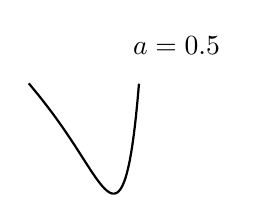
\begin{tikzpicture}[line join=round, scale=0.4]
\mydrawxy{-3}{3}{-2}{3}
\draw[thick,domain=-2:1.5,samples=200] plot (\x,{(0.5)*exp(2*\x)+(0.5-2)*exp(\x)-\x});
\coordinate[label=right:{$a=0.5$}] (t) at (1,3);
\end{tikzpicture}
\end{minipage}
\begin{minipage}{.32\textwidth}
\centering
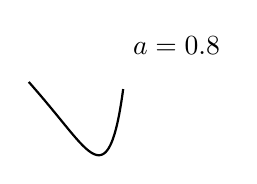
\begin{tikzpicture}[line join=round, scale=0.4]
\mydrawxy{-3}{3}{-2}{3}
\draw[thick,domain=-2:1,samples=200] plot (\x,{(0.8)*exp(2*\x)+(0.8-2)*exp(\x)-\x});
\coordinate[label=right:{$a=0.8$}] (t) at (1,3);
\end{tikzpicture}
\end{minipage}
\begin{minipage}{.32\textwidth}
\centering
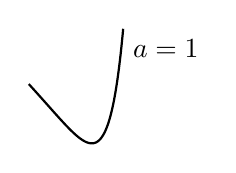
\begin{tikzpicture}[line join=round, scale=0.4]
\mydrawxy{-3}{3}{-2}{3}
\draw[thick,domain=-2:1,samples=200] plot (\x,{(1)*exp(2*\x)+(1-2)*exp(\x)-\x});
\coordinate[label=right:{$a=1$}] (t) at (1,3);
\end{tikzpicture}
\end{minipage}
\end{figure}

\begin{tcolorbox}
本题没有难度。函数形状的讨论都是针对其一阶和二阶导数的分段讨论,讨论的是另两个函数。
\end{tcolorbox}









